\documentclass[12pt]{article}

\usepackage{amssymb, amsmath}
\usepackage{graphicx}
\usepackage{cite}
\usepackage{hyperref}
\usepackage{comment}
\usepackage{xcolor}
\usepackage{spverbatim}

\hypersetup{
     colorlinks   = true,
     citecolor    = blue
}

\def\be{\begin{equation}}
\def\ee{\end{equation}}
\def\bea{\begin{eqnarray}}
\def\eea{\end{eqnarray}}
\def\bes{\begin{equation*}}
\def\ees{\end{equation*}}
\def\beas{\begin{eqnarray*}}
\def\eeas{\end{eqnarray*}}
\def\mcF{\mathcal{F}}
\def\hmcF{\hat{\mathcal{F}}}
\def\mcF{\mathcal{F}}
\def\mcA{\mathcal{A}}
\def\hdel{D}
\def\tr{ \text{Tr}}
\def\td{ \textrm{d}}
\newtheorem{lemma}{Lemma}
\newtheorem{theorem}{Theorem}
\def\nn{\nonumber}
\DeclareMathOperator{\arctanh}{arctanh}

\newcommand{\E}{\mathbb{E}}

\newcommand{\Var}{\mathrm{Var}}

\newcommand{\Cov}{\mathrm{Cov}}

\newcommand{\std}{\mathrm{std}}

\newcommand{\minimise}{\mathrm{minimise}}
\newcommand{\maximise}{\mathrm{maximise}}

\DeclareMathOperator*{\argmax}{arg\,max}
\DeclareMathOperator*{\argmin}{arg\,min}

\newcommand{\COO}{CO\textsubscript{2}}


\hoffset -.6in
\voffset -.2in
\textwidth 16.9cm
\topmargin -1cm
\textheight 23cm


\title{ {\bf How much gas can Europe save this winter?}}

\author{Carmen Li$^{a}$\footnote{c.li@jbs.cam.ac.uk} 
\\ \\  \small \sl  $^a$Cambridge Judge Business School, Trumpington Street, Cambridge CB2 1AG, United Kingdom}

\date{}

\begin{document}

%\maketitle


%\begin{abstract}
%abstract
%\end{abstract}

%\newpage

%\tableofcontents

%\newpage





\section{Introduction}
Following the invasion of Ukraine in February 2022, the European Union (EU) and the United Kingdom (UK) are committed to rapidly decouple from Russian gas, which made up 32\% (158 bcm) of the total gas demand (489 bcm) in 2021 \cite{IEA}. While increasing liquefied natural gas (LNG) imports can ease some of the pressure on replacing the missing energy, curbing demand is another obvious strategy. The industrial and household sectors are the biggest end-users of natural gas in the EU, making up 40\% of the final consumption (for energy use) \textit{each} \cite{Eurostat_sankey}. Cutting gas consumption in industry would inevitably reduce output and slow the economy; households on the other hand may turn down their thermostats without drastically affecting their standard of living. In this note, we estimate how much gas can be saved in Europe by decreasing the setpoint temperature for space heating using the \textit{heating degree-days} (HDD) method, following closely the results of \cite{KOZARCANIN2019368}. 

\section{Heating degree-days}
The heating degree-day method is based on the notion that the \textit{rate} of heat loss $Q_L$ from a building to the surrounding is proportional to the difference between indoor $\theta_I$ and outdoor $\theta_O$ temperature, i.e., 
\be 
Q_L(t) \mathrm{[kW]}=L(t) \mathrm{[kWK^{-1}]} \; \cdot \; \left(\theta_I(t)\mathrm{[K]} - \theta_O(t)\mathrm{[K]} \right) \; , \qquad \theta_I(t) >  \theta_O(t) \; .  
\ee
where $(t)$ signifies the time dependence, and $L$ is the heat loss coefficient which is not necessarily constant as it is affected by disturbances such as opening windows \cite{CIBSE}. Not all the heat lost to the outside needs to be compensated by the heating system though; heat also comes from solar radiation, body heat of the occupants, lights, electrical appliances etc., hence the total heat gain is given by
\be 
Q_G(t) \mathrm{[kW]} = Q_H(t) \mathrm{[kW]} + Q_I(t) \mathrm{[kW]}
\ee 
where $Q_G$ is the total heat gain, $Q_H$ is the heat gain from heating, and $Q_I$ is the internal heat gain from all other sources inside the building as well as solar irradiation. \\
\\
Consider the case of continuous heating to maintain a constant indoor temperature, which is the setpoint temperature $\theta_{sp}$ on the thermostat i.e., $\theta_I(t)=\theta_{sp} > \theta_O(t)$ over a period of time $T$. We may further simplify the model by taking the time averages $\overline{L}$ and $\overline{Q}_I$ instead of the time-varying $L(t)$ and $Q_I(t)$ by assuming that the effect of the fluctuations is evened out when we integrate over a sufficiently long period $T$. Since in a steady state the energy gain must be equal to the energy loss over the period
\bea  
E_H + E_I &=& E_L \\
E_H + \int_0^T \overline{Q}_I \; \td t &=& \int_0^T  \overline{L} \left(\theta_{sp} - \theta_O(t) \right)  \td t 
\eea 
which gives the heating energy as
\be 
E_H = \overline{L} \int_0^T \left(\theta_{sp} - \frac{\overline{Q}_I}{\overline{L}} \right) - \theta_O(t) \; \td t \; . 
\ee
Note that the quantities $\theta_{sp}$, $\overline{Q}_I$ and $\overline{L}$ in the bracket are all constants, so we may define a \textit{threshold temperature}
\be 
\theta_{th} := \theta_{sp} - \frac{\overline{Q}_I}{\overline{L}} \label{threshold_temp}
\ee
and write instead
\be 
E_H = \overline{L} \int_0^T \theta_{th} - \theta_O(t) \; \td t \label{heating_energy}
\ee
i.e., heating is \textit{on} ($E_H>0$) when the outside temperature is below the threshold ($\theta_O(t)<\theta_{th}$), and the heating power is proportional to the temperature gap. This naturally leads to the notion of \textit{heating degree-days} (HDD) over a period $T$ (e.g., a month or a year), which is defined as
\be 
HDD := \frac{1}{\tau}  \int_0^T H \left( \theta_b - \theta_O(t) \right) \; \td t \; , \label{HDD}
\ee
where the factor $1/\tau$ converts the unit of $t$ into days (e.g., $\tau=24$ if temperature is measured hourly, or $\tau=1$ if daily mean temperature is used), and $H(x)$ is a step function which is equal to $x$ if $x>0$ and zero otherwise since we focus only on heating. Using this definition, the heating energy required to keep the indoor space at the constant setpoint temperature $\theta_{sp}$ over $T$ is then simply 
\be 
E_H = \bar{L} \cdot HDD \; ;
\ee 
thus HDD provides a very simple and straightforward method to estimate the demand for space heating at different ambient temperatures.  \\
\\
At national level, equation \eqref{heating_energy} can be scaled accordingly to estimate the annual energy demand from gas for space heating in country $c$ and year $y$ with 
\be  
G(c,y) = \frac{P_g(c,y) \mathcal{L}(c,y)}{\eta_g(c,y)} \; \;   \mathbf{\Theta}^T(c) \; \mathbf{HDD}(c,y)   \label{gas energy}
\ee
where $P_g$ is the population on gas heating, $\mathcal{L}$ is the coefficient that measures the average space heat \textit{energy} loss per person per degree-day, $\eta_g$ is the average efficiency of the gas boilers, $\mathbf{\Theta}$ is a binary vector that indicates which \textit{month} falls in the heating season as given in \cite{KOZARCANIN2019368}, and $\mathbf{HDD}$ is the vector of monthly HDD computed from the thresholds given also in \cite{KOZARCANIN2019368}. Note that all quantities apart from the binary heating season vector $\mathbf{\Theta}$ varies from from year to year. \\
\\
The goal of this exercise is to estimate how much savings in gas can be made under different weather scenarios by reducing the \textit{setpoint} temperature in buildings, treating the \textit{thresholds} reported in \cite{KOZARCANIN2019368} as baseline --- recall from \eqref{threshold_temp} that $\overline{Q}_I$ and $\overline{L}$ are constant mean values and so any change in the setpoint temperature $\theta_{sp}$ will translate directly the to exactly the same change in the threshold temperature $\theta_{th}$. 


\section{Methodology}
In this section we detail the sources of the datasets used in the study and outline each step of the processing of the raw data. The model covers the 28 countries in Europe: AT, BE, BG, CZ, DE, DK, EE, ES, FR, GB, GR, HR, HU, IE, IT, LT, LV, NL, PL, RO, SI, SK, FI, SE, LU, PT, CH, UA. The first 22 countries are covered in \cite{KOZARCANIN2019368} with gas heating; for the 6 remain countries, we assume the threshold of 15 degrees used by Eurostat \cite{Eurostat_hdd}. Gas is not used for space heating in NO but it is included in the HDD analysis for completeness, using also the 15 degrees threshold. 

\subsection{Temperature data}
Ideally, temperature data from the same source as in \cite{KOZARCANIN2019368} should be used for consistency and to avoid systemic bias when taking the difference from the threshold temperature to compute the HDD. However, in the absence of numerical result for the bias adjustment of temperature profiles or further information on the exact procedure for national aggregation, the hourly population weighted temperature data spanning from 1980-01-01 00:00:00 to 2019-12-31 23:00:00 (i.e., 40 years of data) for the 28 countries obtained from \cite{ninja} are used instead. 

\subsubsection*{Calibration}
Since the temperature thresholds reported in \cite{KOZARCANIN2019368} are derived from temperature data from a different source, we need to first \textit{calibrate} our temperature data to the model in order to use these thresholds to compute the HDD. For instance if we compute the average HDD in January from 2008 to 2017 for GB using the temperature data from \cite{ninja} without any calibration and the gas threshold of $\theta_{th}=14.18$ according to \cite{KOZARCANIN2019368}, then we would obtain 324 degree-days, which is 7.6\% higher than the 301 degree-days reported in table 4 in \cite{KOZARCANIN2019368}.\\
\\
The goal is therefore to match with the average monthly HDD reported in \cite{KOZARCANIN2019368} country by country by adjusting the temperature. To proceed, let us assume a simple affine relation between the unknown target temperature $\theta^p_t$ and the data obtained from renewables.ninja  $\theta^n_t$ at each time step $t$, i.e., 
\be 
\theta^p_t = \alpha \theta^n_t + \beta \;.  \label{temp_adj}
\ee
where $\alpha$ and $\beta$ are the coefficients to be determined. We have dropped the country label $c$ since it is clear that this is done for each country. Substituting this into \eqref{HDD}, it can be deduced that for month $m$ during high winter when the temperature is \textit{always} below the threshold and so the step function in \eqref{HDD} can be omitted, the difference in the mean HDD $\overline{HDD}^n_m$ computed directly using the ninja temperature $\theta^n_t$  and the target $\overline{HDD}_m^p$ is given by
\be 
\Delta \overline{HDD}_m:= \overline{HDD}^n_m - \overline{HDD}^p_m = \frac{\alpha -1}{\tau} \sum_{t\in m} \theta^n_t  + \frac{\beta \bar{T}}{\tau} \; . 
\label{temp_linear_regression}
\ee
where $t\in m$ means time steps that belong to the month $m$, $\tau=24$ since our data has hourly resolution, and $\bar{T}$ is the average number of time steps in month $m$, which is only non-trivial for February. Since $\Delta \overline{HDD}_m$ and the sum over ninja temperature can be computed directly for the high winter months, we can use ordinary least square (OLS) to determine the estimates $\hat{\alpha}$ and $\hat{\beta}$ for $\alpha$ and $\beta$. Ideally, only the coldest months where the outside temperature never crosses the threshold $\theta_th$ should be considered in the regression in order to avoid the nonlinearity introduced by the step function $H$; however this is not possible in the warmer countries like Spain (ES), where the coldest three months are used. For the three countries BG, FR and BG where heating from electricity is also modelled in \cite{KOZARCANIN2019368}, the mean HDD is taken to be the weighted sum from gas and electricity heating according to the proportion shown in figure 1 in the paper. For LU and UA which are were included in the study, we use the estimates for DE and BE, and PL and RO respectively by taking the averages to calibrate their temperature. The values of $\hat{\alpha}$ and $\hat{\beta}$ for each country are summarised in table \ref{table:temp_adj} below, along with some indicative performance metrics of the regression model. Evidently, the adjustments are not significant with $\hat{\alpha} \approx 1$ and $|\hat{\beta}|<2$ for all countries. 

\begin{table}[h!]
\centering
\begin{tabular}{l|lllll}
country & \# samples & correlation        & $\hat{\alpha}$             & $\hat{\beta}$          & $\sigma_{HDD}$ \\ \hline
AT & 4          & -0.98       & 0.92  & 1.61      & 8.85              \\
BE & 4          & -0.85       & 0.91  & 1.70      & 6.08              \\
CZ & 4          & -0.71       & 0.95  & 1.57      & 2.39              \\
DE & 4          & -0.82       & 0.90  & 1.57      & 7.33              \\
DK & 6          & 0.10        & 1.00  & 0.72      & -2.53             \\
EE & 5          & -0.79       & 0.92  & 0.94      & -7.57             \\
GB & 5          & 0.05        & 1.00  & 0.72      & -1.71             \\
GR & 4          & -0.61       & 0.98  & 0.23      & -1.43             \\
HR & 5          & -0.88       & 0.96  & 1.11      & -8.11             \\
HU & 4          & -0.93       & 0.93  & 1.67      & 4.75              \\
IE & 4          & -0.02       & 1.00  & 0.39      & -3.74             \\
IT & 5          & -0.87       & 0.90  & 1.94      & 6.92              \\
LT & 6          & -0.92       & 0.89  & 1.69      & -2.91             \\
LV & 5          & -0.97       & 0.90  & 1.72      & -1.04             \\
NL & 5          & -0.72       & 0.94  & 0.91      & 10.00             \\
PL & 6          & -0.92       & 0.87  & 1.52      & 11.39             \\
RO & 3          & -0.43       & 0.96  & 1.05      & -8.58             \\
SI & 4          & -0.67       & 0.97  & 0.80      & 13.28             \\
SK & 4          & -0.96       & 0.92  & 1.23      & -16.11            \\
CH & 5          & -0.92       & 0.87  & 0.63      & 0.92              \\
FI & 7          & -0.78       & 0.90  & 0.46      & 25.11             \\
NO & 7          & -0.75       & 0.90  & 1.61      & -8.38             \\
SE & 6          & -0.55       & 0.95  & 0.41      & -1.93             \\
PT & 3          & -0.90       & 0.83  & 1.78      & -2.61             \\
BG & 5          & -0.86       & 0.98  & -0.48     & -7.51             \\
ES & 3          & 0.78        & 1.04  & 1.00      & 61.29             \\
FR & 5          & -0.58       & 0.96  & 0.73      & 17.68            
\end{tabular}
\caption{Table summarising the estimates for the calibration parameters alongside a summary of the regression model for each country, including the number of points (months) considered, their Pearson correlation, and $\sigma_{HDD}$ is the annual deviation from the target HDD post-calibration summed over the heating months.} \label{table:temp_adj}
\end{table}

\subsubsection*{Weather year scenarios}
Using the adjusted temperature, we may compute the annual HDD over the heating season from 1980 to 2019 for each country. The 40 annual samples are then clustered into three weather categories --- mild, normal and hard using agglomerative clustering with complete linkage, and the cluster median is chosen as the representative year for the weather scenario. On top of these three scenarios, we also consider four extreme scenarios --- the mildest and the hardest years with the smallest and largest HDD within the 40-year period, as well as two peak years when the coldest 7-day period occurred over the full period from 1980--2019 (peak80), and the latter half from 2000--2019 (peak00). Note that while the mildest, mild, normal, hard and hardest years are always distinct, the peak years may coincide with each other or with the hard or hardest years. Table \ref{table:clusters_size} shows the number of years in each of the three clusters, while table \ref{table:rep_year} summaries the representative year for each scenario.  

\begin{table}[h!]
\centering
\begin{tabular}{l|lll}
country   & mild & normal & hard \\ \hline
AT & 13   & 22     & 5    \\
BE & 15   & 20     & 5    \\
BG & 2    & 18     & 20   \\
CZ & 5    & 8      & 27   \\
DE & 5    & 19     & 16   \\
DK & 7    & 9      & 24   \\
EE & 18   & 19     & 3    \\
ES & 18   & 11     & 11   \\
FR & 11   & 23     & 6    \\
GB & 17   & 15     & 8    \\
GR & 3    & 14     & 23   \\
HR & 2    & 14     & 24   \\
HU & 15   & 19     & 6    \\
IE & 28   & 9      & 3    \\
IT & 10   & 20     & 10   \\
LT & 11   & 24     & 5    \\
LV & 11   & 24     & 5    \\
NL & 18   & 8      & 14   \\
PL & 15   & 20     & 5    \\
RO & 7    & 28     & 5    \\
SI & 15   & 2      & 23   \\
SK & 2    & 16     & 22   \\
FI & 5    & 22     & 13   \\
SE & 24   & 9      & 7    \\
LU & 22   & 12     & 6    \\
PT & 3    & 20     & 17   \\
CH & 9    & 24     & 7    \\
UA & 6    & 7      & 27   \\
NO & 19   & 14     & 7   
\end{tabular}
\caption{The number of years in each weather cluster. } \label{table:clusters_size}
\end{table}


\begin{table}[h!]
\centering
\begin{tabular}{l|lllllll}
country   & mildest & mild & normal & hard & hardest & peak80 & peak00 \\ \hline
AT & 2014    & 1994 & 1982   & 1985 & 1996    & 1985   & 2012   \\
BE & 2014    & 2002 & 1992   & 2010 & 1985    & 1987   & 2012   \\
BG & 2019    & 2014 & 1994   & 1984 & 2003    & 2012   & 2012   \\
CZ & 2014    & 2000 & 2013   & 1985 & 1996    & 1996   & 2006   \\
DE & 2014    & 2019 & 1999   & 1991 & 1996    & 1987   & 2012   \\
DK & 2014    & 1990 & 1991   & 1987 & 2010    & 1987   & 2012   \\
EE & 2015    & 2007 & 1998   & 1987 & 1985    & 1987   & 2011   \\
ES & 1989    & 2019 & 1988   & 1999 & 2005    & 1985   & 2012   \\
FR & 2014    & 2019 & 1982   & 1980 & 1985    & 1985   & 2012   \\
GB & 2014    & 2019 & 2012   & 1987 & 2010    & 1982   & 2010   \\
GR & 2014    & 2019 & 1999   & 1980 & 1983    & 1987   & 2002   \\
HR & 2014    & 2014 & 1989   & 1984 & 1996    & 1985   & 2012   \\
HU & 2014    & 1989 & 1995   & 1980 & 1996    & 1996   & 2006   \\
IE & 2002    & 1990 & 2001   & 1985 & 2010    & 2010   & 2010   \\
IT & 2014    & 2016 & 1992   & 1986 & 1980    & 1985   & 2012   \\
LT & 1990    & 2015 & 1994   & 2010 & 1985    & 2006   & 2006   \\
LV & 1990    & 2019 & 2002   & 2010 & 1985    & 1987   & 2006   \\
NL & 2014    & 1999 & 1995   & 1986 & 1996    & 1987   & 2012   \\
PL & 2019    & 2018 & 1982   & 1987 & 1996    & 1987   & 2010   \\
RO & 2019    & 2008 & 1992   & 1987 & 1985    & 2012   & 2012   \\
SI & 2014    & 2014 & 2001   & 2010 & 1980    & 1985   & 2012   \\
SK & 2014    & 2014 & 1994   & 1991 & 1996    & 1987   & 2012   \\
FI & 2015    & 1989 & 1991   & 1981 & 1985    & 1987   & 2011   \\
SE & 2000    & 2006 & 1993   & 1987 & 1985    & 1987   & 2010   \\
LU & 2014    & 1990 & 1997   & 1987 & 1996    & 1985   & 2012   \\
PT & 1995    & 1997 & 1988   & 1992 & 2005    & 1985   & 2009   \\
CH & 2014    & 1994 & 2000   & 1995 & 2010    & 1985   & 2012   \\
UA & 1990    & 2008 & 2005   & 1980 & 1987    & 2006   & 2006   \\
NO & 2000    & 2017 & 1988   & 1980 & 2010    & 1987   & 2010  
\end{tabular}
\caption{Representative year for each scenario.} \label{table:rep_year}
\end{table}

\subsection{From HDD to gas demand}
Recall from \eqref{gas energy} that in order to convert HDD into gas energy demand for space heating, we also need the parameters $P_g$, $\mathcal{L}$ and $\eta_g$, all of which change with time. Moreover, their values cannot be obtained directly from any publicly available sources. For instance, instead of the population on gas heating $P_g(c,y)$, only total population $P(c,y)$ is available from Eurostat \cite{Eurostat2}, though we may assume $P_g(c,y)=P(c,y) \cdot f_g(c)$ by introducing another factor $f_g(c)$, which is the fraction of population on gas heating and may be assumed to be constant since progress on transition from gas boilers to heat pumps has been slow in most countries. On the other hand, the energy conversion factor $\mathcal{L}(c,y)$ and the average boiler efficiency $\eta_g(c,y)$ are simply not available. However, since we \textit{can} obtain historical data for the annual gas demand for residential space heating $G_E$ on the left hand side of \eqref{gas energy} also from Eurostat \cite{Eurostat1}\footnote{The residential space heating gas demand data for CH are obtained from the Swiss Federal Office of Energy \cite{SFOE}}, we may rewrite \eqref{gas energy} as
\be 
G_E(c,y) = P(c,y) \cdot \tilde{\mathcal{L}}^{20}(c) \cdot I_\eta^{20}(c,y) \cdot {HDD}(c,y)  \label{gas_model}
\ee
to model the gas demand, where
\be
\tilde{\mathcal{L}}^{20}(c) = \frac{f_g(c) \mathcal{L}(c, 2020)}{\eta_g(c, 2020)}
\ee
is the constant of proportionality relating the gas energy demand and the annual HDD during the heating season in the year 2020, and $I_\eta^{20}(c,y)$ is the overall efficiency index relative to 2020 which accounts for changes in both the boiler efficiency and energy efficiency of buildings. Note that we also assume that the rate of improvement in efficiency is the same for both the building itself and the appliances inside the building that contribute to internal heat gain, and so the ratio $\overline{Q}_I/\overline{L}$ in \eqref{threshold_temp} remains the same and so that a one degree change in the set point temperature $\theta_{sp}$ still translates to one degree change in the heating threshold temperature $\theta_{th}$. \\
\\
To estimate the efficiency indices $I_\eta^{20}(c,y)$, we use the \textit{unit consumption per m$^2$ for space heating with climatic corrections} data set from \cite{ODYSSEE}. Because efficiency \textit{improves} over time, not only for gas boilers but also better insulation in buildings can reduce heat loss, $I_\eta^{20}(c,y)$ should be monotonically decreasing, and we may assume that it is also smoothly decreasing. We therefore try and fit the following models:
\bea
\eta^{ed}(y) &=& a_1 \exp(-b_1y) + c \\
\eta^{meg}(y) &=& c_2 - a_2 \exp(b_2y) \\
\eta^a(y) &=& a_3 y+c_3
\eea
i.e., exponential decay (\textit{ed}), minus exponential growth (\textit{meg}), and affine ($a$) models for each country using the least square method, and choose the model that best fits the data. Figure \ref{fig:efficiency_index_AT} illustrates the example for AT where the exponential decay model is the best fit with $\hat{a}_1=4.30$, $\hat{b}_1=0.22$ and $\hat{c}_1=13.69$ before normalisation. Table \ref{table:efficiency_index} shows the efficiency index $I_\eta^{20}(c,y)$ from 2015 to 2022. For NO, BE and UA where efficiency data are not available, we take the EU average. Finally, we may now estimate the constant $\tilde{\mathcal{L}}^{20}(c)$ in \eqref{gas_model} using OLS linear regression; it has unit [TJ/capita/HDD] and the results are listed in table \ref{table:L}. The gas demand computed from \ref{gas_model} with all the parameters given above is therefore measured in united [TJ], which can be concerted into volume using 1 bcm = 37 PJ for Russian natural gas.


\begin{figure}[h!]
\centering
	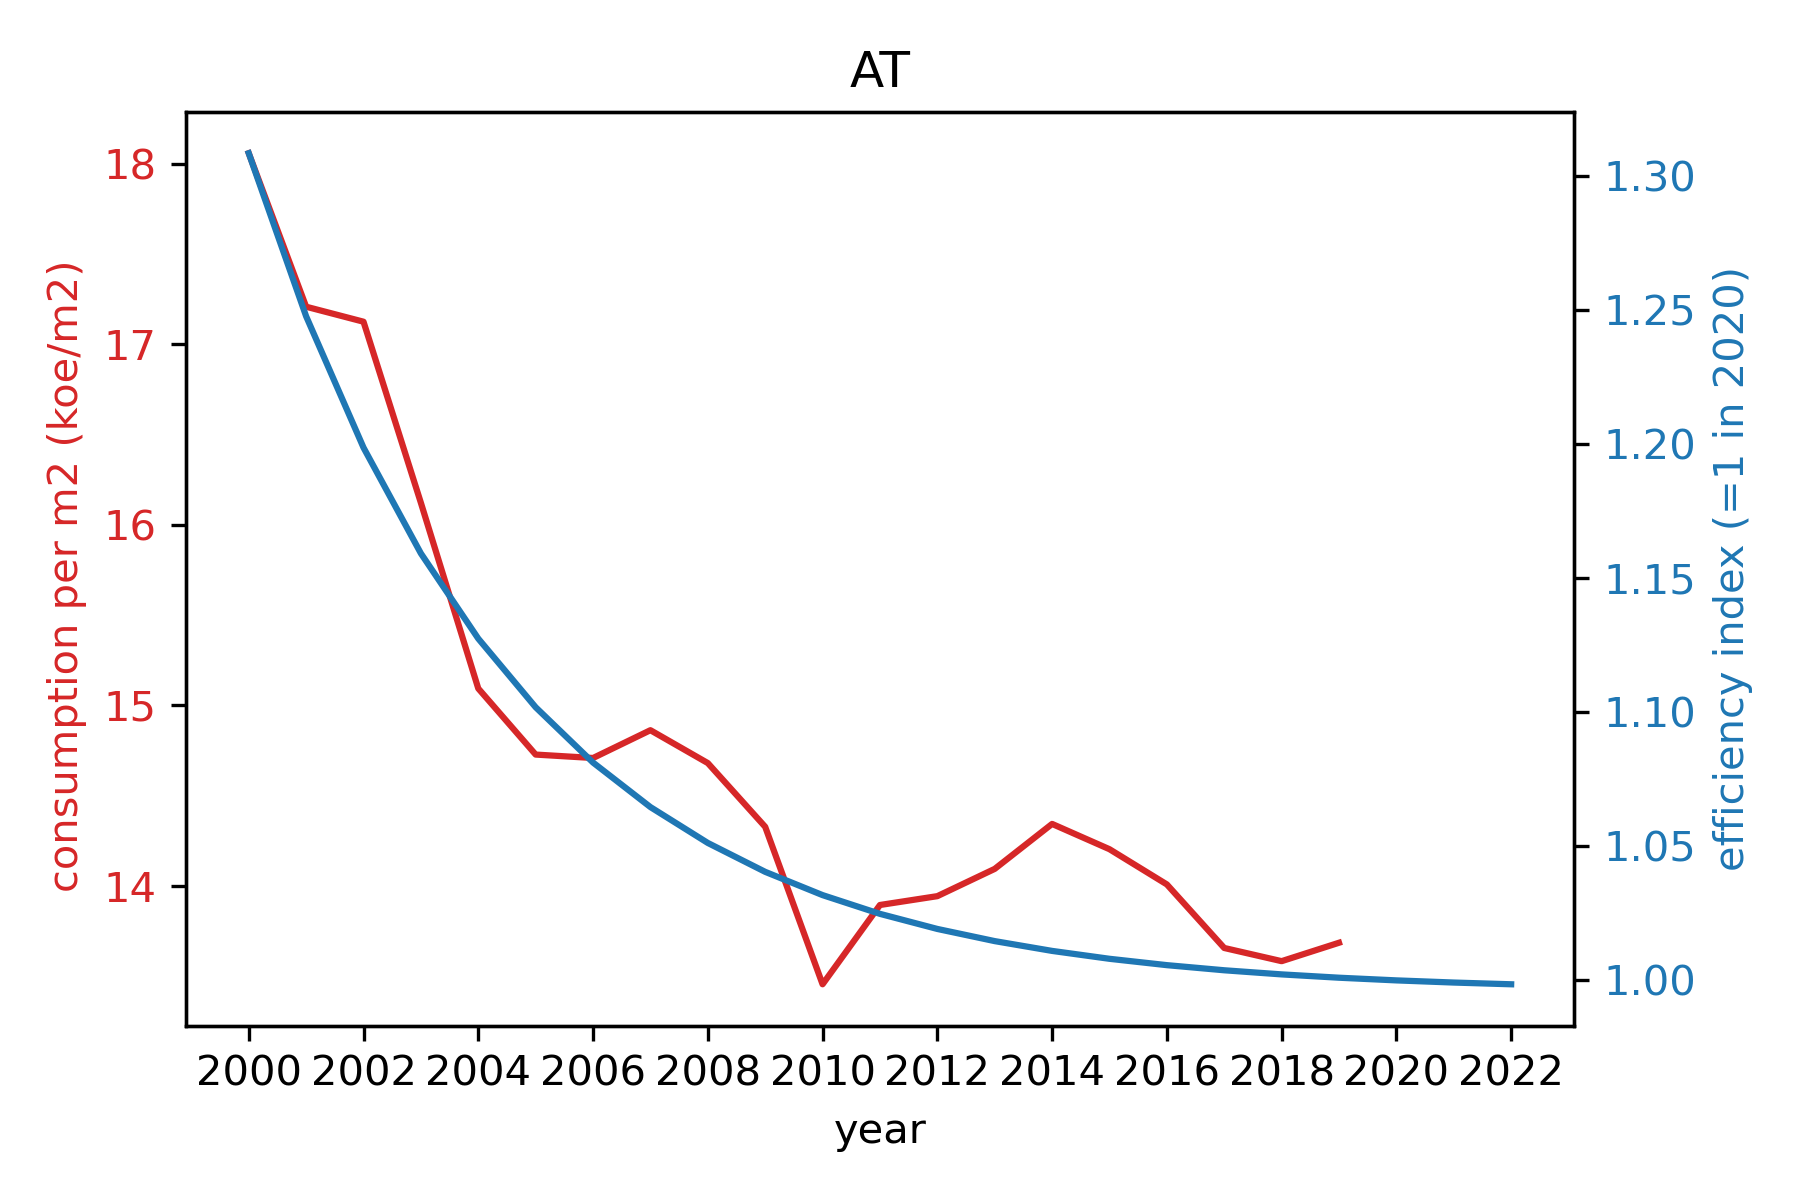
\includegraphics[width=0.6\textwidth]{efficiency_index_AT}
	\caption{Exponential decay model for efficiency index of AT. } \label{fig:efficiency_index_AT}
\end{figure}


\begin{table}[h!]
\centering
\begin{tabular}{l|lllllllll}
country & 2015  & 2016  & 2017  & 2018  & 2019  & 2020 & 2021  & 2022  & $\sigma_{I_\eta}$ \\ \hline
AT      & 1.008 & 1.006 & 1.004 & 1.002 & 1.001 & 1    & 0.999 & 0.999 & 0.021       \\
BG      & 1.009 & 1.007 & 1.005 & 1.003 & 1.002 & 1    & 0.998 & 0.997 & 0.044       \\
HR      & 1.121 & 1.098 & 1.075 & 1.051 & 1.026 & 1    & 0.973 & 0.946 & 0.020       \\
CY      & 1.043 & 1.031 & 1.021 & 1.013 & 1.006 & 1    & 0.995 & 0.991 & 0.135       \\
CZ      & 1.035 & 1.026 & 1.019 & 1.012 & 1.006 & 1    & 0.995 & 0.990 & 0.031       \\
DK      & 1.008 & 1.005 & 1.003 & 1.002 & 1.001 & 1    & 1.000 & 0.999 & 0.025       \\
EE      & 1.046 & 1.037 & 1.027 & 1.018 & 1.009 & 1    & 0.991 & 0.983 & 0.042       \\
FI      & 1.152 & 1.132 & 1.107 & 1.078 & 1.042 & 1    & 0.949 & 0.888 & 0.017       \\
FR      & 1.077 & 1.060 & 1.043 & 1.028 & 1.013 & 1    & 0.987 & 0.976 & 0.014       \\
DE      & 1.059 & 1.045 & 1.032 & 1.020 & 1.009 & 1    & 0.992 & 0.984 & 0.043       \\
GR      & 1.017 & 1.009 & 1.004 & 1.002 & 1.001 & 1    & 1.000 & 0.999 & 0.060       \\
HU      & 1.054 & 1.043 & 1.032 & 1.022 & 1.011 & 1    & 0.989 & 0.978 & 0.008       \\
IE      & 1.062 & 1.042 & 1.027 & 1.016 & 1.007 & 1    & 0.995 & 0.991 & 0.040       \\
IT      & 1.059 & 1.053 & 1.045 & 1.034 & 1.019 & 1    & 0.974 & 0.940 & 0.020       \\
LV      & 1.148 & 1.116 & 1.085 & 1.056 & 1.027 & 1    & 0.974 & 0.948 & 0.051       \\
LT      & 1.030 & 1.020 & 1.013 & 1.007 & 1.003 & 1    & 0.998 & 0.996 & 0.039       \\
LU      & 1.019 & 1.012 & 1.008 & 1.004 & 1.002 & 1    & 0.999 & 0.998 & 0.059       \\
NL      & 1.128 & 1.100 & 1.073 & 1.048 & 1.023 & 1    & 0.978 & 0.957 & 0.027       \\
PL      & 1.151 & 1.125 & 1.098 & 1.068 & 1.035 & 1    & 0.962 & 0.921 & 0.040       \\
PT      & 1.091 & 1.069 & 1.049 & 1.031 & 1.015 & 1    & 0.987 & 0.975 & 0.143       \\
RO      & 1.007 & 1.005 & 1.003 & 1.002 & 1.001 & 1    & 0.999 & 0.999 & 0.071       \\
SK      & 1.046 & 1.034 & 1.024 & 1.015 & 1.007 & 1    & 0.994 & 0.989 & 0.054       \\
SI      & 1.156 & 1.122 & 1.089 & 1.057 & 1.028 & 1    & 0.974 & 0.948 & 0.019       \\
ES      & 1.169 & 1.138 & 1.106 & 1.072 & 1.037 & 1    & 0.962 & 0.921 & 0.073       \\
SE      & 1.091 & 1.071 & 1.053 & 1.034 & 1.017 & 1    & 0.984 & 0.968 & 0.046       \\
CH      & 1.122 & 1.098 & 1.073 & 1.049 & 1.024 & 1    & 0.976 & 0.952 & 0.021       \\
GB      & 1.086 & 1.065 & 1.046 & 1.029 & 1.014 & 1    & 0.987 & 0.976 & 0.032       \\
EU      & 1.078 & 1.061 & 1.045 & 1.029 & 1.014 & 1    & 0.986 & 0.973 & 0.020       \\
EU28    & 1.096 & 1.076 & 1.056 & 1.037 & 1.018 & 1    & 0.982 & 0.965 & 0.018       \\
NO      & 1.078 & 1.061 & 1.045 & 1.029 & 1.014 & 1    & 0.986 & 0.973 & 0.020       \\
BE      & 1.078 & 1.061 & 1.045 & 1.029 & 1.014 & 1    & 0.986 & 0.973 & 0.020       \\
UA      & 1.078 & 1.061 & 1.045 & 1.029 & 1.014 & 1    & 0.986 & 0.973 & 0.020      
\end{tabular}
\caption{Efficiency index $I_\eta^{20}$ (=1 in 2020). $\sigma_{I_\eta}$ is the scaled standard error of residuals from the curve fitting. } \label{table:efficiency_index}
\end{table}


\begin{table}[h!]
\centering
\begin{tabular}{l|lll}
country & \# points & $\hat{\tilde{\mathcal{L}}}^{20}$   & $\sigma_{\tilde{\mathcal{L}}^{20}}$ \\ \hline
AT      & 10        & 2.472 & 0.033    \\
BE      & 4         & 5.694 & 0.172    \\
BG      & 10        & 0.113 & 0.009    \\
CZ      & 5         & 2.063 & 0.026    \\
DE      & 10        & 4.239 & 0.134    \\
DK      & 5         & 1.563 & 0.043    \\
EE      & 10        & 0.533 & 0.027    \\
ES      & 10        & 1.023 & 0.038    \\
FR      & 10        & 3.206 & 0.067    \\
GB      & 9         & 6.975 & 0.101    \\
GR      & 6         & 1.119 & 0.085    \\
HR      & 10        & 1.282 & 0.037    \\
HU      & 5         & 4.268 & 0.172    \\
IE      & 5         & 3.689 & 0.088    \\
IT      & 5         & 7.380 & 0.100    \\
LT      & 3         & 0.582 & 0.030    \\
LV      & 10        & 0.426 & 0.028    \\
NL      & 10        & 7.965 & 0.073    \\
PL      & 5         & 0.766 & 0.037    \\
RO      & 5         & 1.457 & 0.071    \\
SI      & 10        & 0.633 & 0.025    \\
SK      & 5         & 3.023 & 0.106   
\end{tabular}
\caption{Summary of the OLS estimate of $\tilde{\mathcal{L}}^{20}$ (in TJ of gas energy per capita per HDD) and its uncertainty $\sigma_{\tilde{\mathcal{L}}^{20}}$ (from the standard error). \# points indicates how many points (years) are used in the OLS linear regression.} \label{table:L}
\end{table}

\section{Uncertainty}
In this section we evaluate the error of the final gas demand estimate by accounting for the uncertainty of the modelled parameters in \eqref{gas_model}, namely $\tilde{\mathcal{L}}^{20}$, $HDD$ and $I_\eta^{20}$ as shown in the tables above. Based on \eqref{gas_model}, the uncertainty of $G_E$ is thus given by
\be 
\sigma_{GE}^2 =  \left(P \cdot HDD \cdot I_\eta^{20} \right)^2  {\sigma^2_{\tilde{\mathcal{L}}^{20}}} +
 \left(P \cdot \tilde{\mathcal{L}}^{20}\cdot I_\eta^{20} \right)^2  {\sigma^2_{HDD}}  +
 \left(P \cdot \tilde{\mathcal{L}}^{20} \cdot {HDD} \right)^2  {\sigma_{I_\eta}}^2 \; . 
\ee
$\sigma_{HDD}$ for LU and UA are taken to be the maximum value of $\sigma_{HDD}$ from BE and DE and PL and RO respectively.  

\section{Result and analysis}
Estimates for the gas demand in billion cubic meters (bcm) for $\pm 5 C$ change in $\theta_{sp} (c)$ in steps of $0.5C$ for the 28 countries and the 7 weather scenarios can be found in the ``output'' directory under the ``eurostat'' subdirectory. The savings in gas in billion cubic meters (bcm) for the whole Europe (summed over the 28 countries) are summarised in figure \ref{fig:delta_gas_demand_bcm_whole_europe}. The relationship between savings and changes in the setpoint temperature is not exactly linear due to the step function in \eqref{HDD}, and the differences between weather scenarios are not huge. 
\begin{figure}[h!]
\centering
	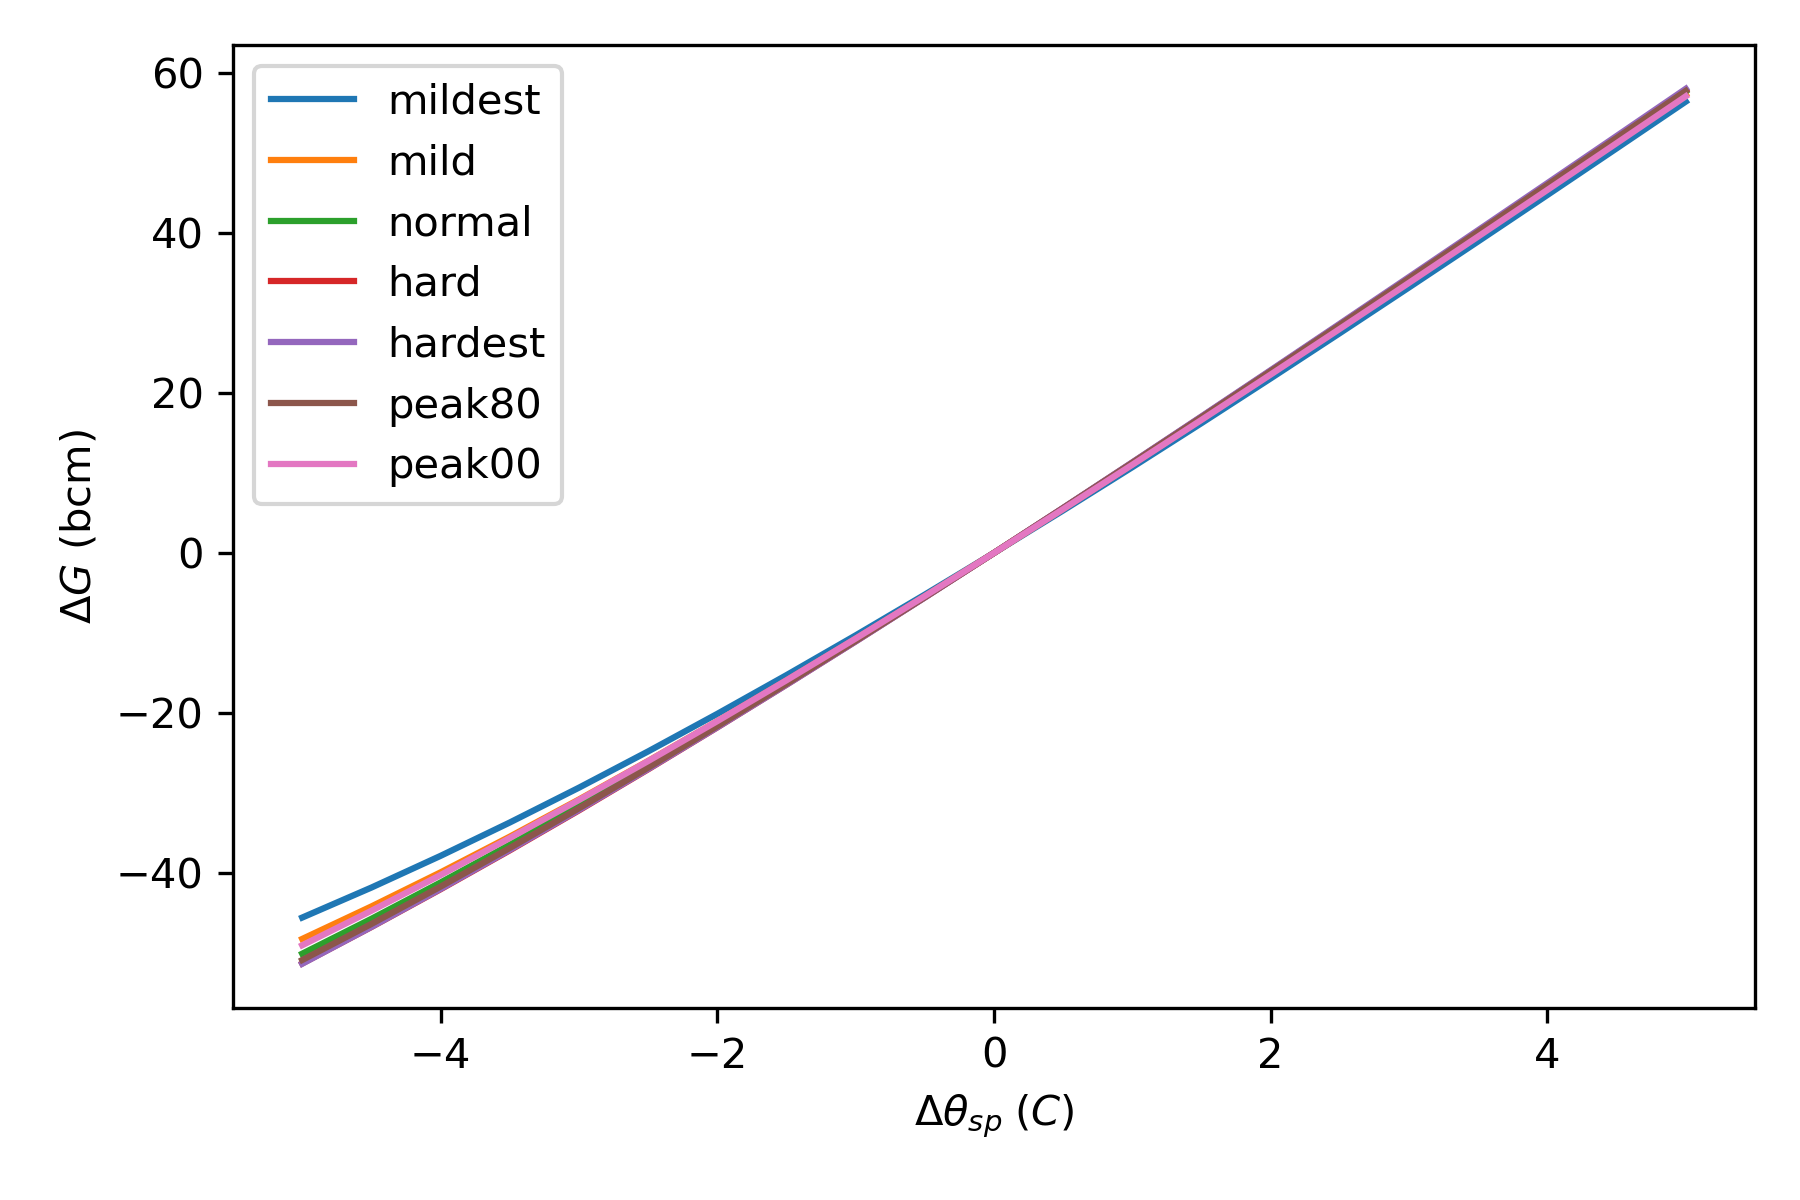
\includegraphics[width=0.6\textwidth]{delta_gas_demand_bcm_whole_europe}
	\caption{Change in gas demand in Europe with respect to change in setpoint temperature under different weather scenarios. } \label{fig:delta_gas_demand_bcm_whole_europe}
\end{figure}


\section{Service sector and the JRCIDEES dataset}
So far our discussion has been focussing on space heating in households. Similar calculation can be done for buildings in the commercial sector as well, assuming the same evolution in the efficiency index as the household sector, by replacing $G_E$ in \eqref{gas_model} with the space heating gas demand data for the service sector from \cite{JRC}, which covers 2000-2015, and estimate the coefficient $\tilde{\mathcal{L}'}^{20}$ using OLS, and repeat the sensitivity analysis with different threshold temperatures. The results are given in the excel files with the prefix ``COM" in the ``JRC'' subdirectory inside the ``output'' directory. Since the dataset also contains annual gas demand for space heating in households, we also computed a separate set of results using the JRCIDEES data; the results can be found in excel files with the prefix ``households'' and may be compared to the results computed from the Eurostat data. Note that the JRCIDEES dataset is older, although it has two more years of data, and UA is also not covered. 

 
\newpage

\bibliography{references}
\bibliographystyle{ieeetr}  



 
\end{document}

